\documentclass[10pt,a4paper]{report}
\usepackage[utf8x]{inputenc}
\usepackage{ucs}
\usepackage{amsmath}
\usepackage{amsfonts}
\usepackage{amssymb}
\usepackage{makeidx}
\usepackage{graphicx}
\usepackage[brazil]{babel}
\usepackage{hyperref}
\usepackage{pdfpages}
\usepackage{enumerate}
\author{Vagner Clementino}
\title{Relatório de Progresso do Mestrado\\
	Vagner Clementino}
	\makeindex

\begin{document}
\maketitle

\chapter{Objetivo do Documento}
\label{sec:objetivo}

O presente documento tem por objetivo subsidiar o pedido de prorrogação de
defesa do aluno Vagner Clementino dos Santos. Ele detalha o histórico da vida
acadêmica do aluno, descreve a situação atual das atividades da dissertação e
apresenta um plano de trabalho visando a conclusão da pesquisa. O texto se
dedica ainda em apresentar a motivação que embasam o adiamento da defesa.

\chapter{Histórico do Aluno}
\label{sec:historico}

O aluno Vagner Clementino dos Santos ingressou no Programa de Pós Graduação em
Ciência da Computação (PPGCC) no segundo semestre de 2014 sob a
o\-ri\-en\-ta\-ção do professor Rodolfo F. Resende. Trata-se de um aluno de
tempo parcial que divide o seu tempo como aluno de mestrado e analista de
desenvolvimento na Empresa de Informática de Belo Horizonte (PRODABEL), onde
trabalha por 40 horas semanais.

O período 2014/2, primeiro semestre como aluno do PPGCC, foi devotado às
disciplinas do programa, sendo que a proposta de dissertação estava em avaliação
com base na literatura em Engenharia de Software. No período 2015/1 a proposta
de dissertação foi materializada e apresentada ao Colegiado em maio de 2015. Sob
o título de \textit{UMA LINGUAGEM PARA MODELAGEM CONCEITUAL EM XBRL} foi
proposto o desenvolvimento de uma linguagem conceitual para a XBRL
(\textit{eXtensible Business Reporting Language})\footnote{\url{www.xbrl.org}}
que é uma linguagem para divulgação e intercâmbio de informações financeiras
baseada em XML\@. O tema foi escolhido por se tratar de um assunto de interesse
no contexto do trabalho do mestrando. Contudo, durante o desenvolvimento da
referida proposta, a conjunção de fatores que a sustentava deixou de existir.
Assim, por iniciativa do próprio aluno, foi realizada uma mudança de tema
mediante a apresentação de um novo projeto de dissertação.

Em dezembro de 2015 foi apresentada uma nova proposta denominada \textit{UM
		ESTUDO DE FERRAMENTAS DE GERENCIAMENTO DE REQUISIÇÃO DE MUDANÇA} que, em
	síntese, visa investigar e contribuir na questão de como este tipo de ferramenta
	vem sendo melhorada ou estendida no contexto da transformação do processo de
	desenvolvimento de software, bem como da manutenção, de um modelo tradicional
	para um outro que incorpora práticas dos agilistas. As manutenções de software
	podem ser divididas em \textit{Corretiva, Adaptativa, Perfectiva e
		Preventiva}~\cite{Lientz:1980:SMM:601062,159342}. A \textit{ISO
		14764}~\cite{1703974} propõe a divisão da tarefa de manutenção nos quatro
	tipos descritos anteriormente e propõe que exista um elemento denominado
	Requisição de Mudança que representa as ca\-rac\-te\-rís\-ti\-cas comuns a todas
	aqueles tipos de manutenção. As Ferramentas de Gerenciamento de Requisições de
	Mudança são aquelas utilizadas pelas organizações para \textit{gerenciar as
		Requisições de Mudança}\cite{1703974} em Software. Após as correções
	solicitadas pelo revisor a proposta foi reapresentada em 03/07/2016 sendo desta
	vez aprovada.

	No tocante às disciplinas, vale evidenciar que os créditos necessários à
	integralização do curso já foram obtidos faltando apenas aqueles relativos à
	Elaboração de Trabalho Final conforme disposto na Tabela~\ref{tab:historico}.

	\begin{table}[htb]
		\centering
		\resizebox{\textwidth}{!}{%}
		\begin{tabular}{llllllll}
			\hline
			Período & Turma & Nome Atividade &
			Nota & Conceito & Sit. Final & Créditos & Integralizado \\ \hline
			2014/2  & DIP DCC831PG9 & TÓPICOS ESPECIAIS EM CIÊNCIA DA COMPUTAÇÃO & 80
			& B    & A         & 4        & Sim           \\
			2014/2  & DIP DCC890PG  & TÓPICOS EM ENGENHARIA DE SOFTWARE        & 91
			& A    & A         & 4        & Sim           \\
			2015/1  & DIP DCC865PG  & PROJETO E ANALISE DE ALGORITMOS          & 70
			& C    & A         & 4        & Sim           \\
			2015/1  & DIP DCC890PG2 & TÓPICOS EM ENGENHARIA DE SOFTWARE        & 73
			& C    & A         & 4        & Sim           \\
			2015/2  & DIP DCC890PG1 & TÓPICOS EM ENGENHARIA DE SOFTWARE        & 81
			& B    & A         & 4        & Sim           \\
			2016/1  & DIP DCC890PG1 & TÓPICOS EM ENGENHARIA DE SOFTWARE        & 60
			& D    & A         & 4        & Sim           \\
			2016/1  & DIP DCC904PG  & ESTAGIO EM DOCÊNCIA I                    & 97
			& A    & A         & 2        & Sim           \\
			2016/1  & ETF GER000    & ELABORAÇÃO DE TRABALHO FINAL             &
			&      &           & 0        & Sim           \\
			2016/2  & ETF GER000    & ELABORAÇÃO DE TRABALHO FINAL             &
			&      &           & 0        & Sim           \\ \hline
		\end{tabular}
		}
		\caption{Histórico Escolar do Aluno}
	\label{tab:historico}
	\end{table}

	\chapter{Situação Atual do Trabalho}
	\label{situacao-atual}

	O trabalho de dissertação encontra-se em finalização e é composto pelas etapas
	listadas a seguir.

	\begin{enumerate}[(i)]
		\item Mapeamento Sistemático da Literatura~\cite{keele2007guidelines}
		\item Caracterização das Ferramentas de Suporte de Problemas de Software
			(FGRM)
		\item Pesquisa (Survey) com os
			desenvolvedores~\cite{wohlin2012experimentation}
		\item Recomendações de Melhorias para as FGRM's
		\item Esforços de Implementação
	\end{enumerate}

	Em comparação ao Projeto de Dissertação apresentado a este Colegiado é possível
	observar que a etapa ``Recomendações de Melhorias para as FGRM's'' foi incluída.
	Nas próximas subseções é detalhado o andamento de cada etapa da dissertação. Não
	obstante, um quadro com visão geral da situação do trabalho pode observado na
	Tabela~\ref{tab:situacao}

	\begin{table}[ht]
		\centering
		\resizebox{\textwidth}{!}{%
			\begin{tabular}{|c|l|c|}
				\hline
				\textbf{\#} & \multicolumn{1}{c|}{\textbf{Descrição}} & \textbf{Situação}  \\ \hline
				01 & Caracterização das FGRM	 	& \textit{Feito} \\ \hline
				02 & Mapeamento Sistemático da Literatura & \textit{Feito} \\ \hline
				03 & Levantamento (survey) com profissionais & \textit{Feito} \\ \hline
				04 & Recomendação de melhorias para as FGRM's & \textit{Em Desenvolvimento} \\ \hline
				05 & Esforços de implementação & \textit{Em Desenvolvimento} \\ \hline
			\end{tabular}%
		}
		\caption{Situação Geral da Dissertação}
		\label{tab:situacao}
	\end{table}

	Tomando com base a Tabela~\ref{tab:situacao} é possível verificar que grande
	parte das atividades necessárias à conclusão da dissertação já foram realizadas.
	Para os itens \textit{1,2 e 3} estamos realizando a revisão final do texto.
	Neste sentido, para concluirmos os itens \textit{4 e 5} que este pedido está
	sendo realizado.

	\subsection{Caracterização das Ferramentas de Gerenciamento de Requisições de
		Mudança (FGRM)}
	\label{subsec:caracterizacao}

	Esta etapa do trabalho consiste em estudo exploratório com o objetivo de
	estabelecer um ``modelo de referência das FGRM's'' o qual identifica as
	fun\-ci\-o\-na\-li\-da\-des mínimas deste tipo de ferramenta. O estudo foi
	realizado com base na leitura da documentação de algumas FGRM's de modo a
	levantar as funções ofertadas por cada um dos sistemas. Os software foram
	escolhidos mediante uma pesquisa (survey) com profissionais envolvidos em
	manutenção de software. A escolha se deu com base em uma lista disponível na
	Wikipédia que compara diversas
	FGRM\footnote{\url{https://en.wikipedia.org/wiki/Comparison_of_issue-tracking_systems}}.

	O resultado deste estudo permite compreender melhor este tipo de ferramenta
	tomando como base as suas funcionalidades. Também é possível propor uma
	classificação dos estudos para as FGRM tendo em vista o conjunto mínimo de
	funções deste tipo de sistema, conforme pode ser observado na
	Subseção~\ref{subsec:revisao_sistematica}. Esta etapa da dissertação foi
	finalizada. O texto do respectivo capítulo está sendo revisado junto com o
	orientador.

	\subsection{Mapeamento Sistemático da Literatura}
	\label{subsec:revisao_sistematica}

	Um \textit{Mapeamento Sistemático da Literatura}, também conhecido como Estudos
	de Escopo (Scoping Studies), tem como objetivos fornecer uma visão geral de
	determinada área de pesquisa, estabelecer se existem evidências de estudos sobre
	determinado tema e fornecer uma indicação da quantidade de trabalho na linha de
	pesquisa sob análise~\cite{keele2007guidelines,wohlin2012experimentation}. Nesta
	dissertação realizamos a classificação dos estudos primários selecionados
	conforme as dimensões de melhoria proposta por Zimmermann e
	outros~\cite{zimmermann2009improving}. Esta etapa do trabalho já foi finalizada
	e os seus resultados foram utilizadas na pesquisa com profissionais (vide
	Subseção~\ref{subsec:survey}). O texto está sendo revisado junto com o
	orientador.

	\subsection{Pesquisa com Profissionais}
	\label{subsec:survey}

	Com o objetivo de coletar os aspectos mais importantes relativo às
	fun\-ci\-o\-na\-li\-da\-des das FGRM's, do ponto de vista dos profissionais
	ligados à manutenção de software, foi realizado um levantamento com questionário
	(survey).  O planejamento e o desenho da pesquisa seguirá as diretrizes
	propostas em Wohlin e outros~\cite{wohlin2012experimentation}. A amostra da
	população de interesse foi coletada com base no estudo proposto por de
	Mello~\cite{de2015investigating}.

	Os questionários foram aplicados e obtivemos um total de 84 respostas. Está
	sendo avaliada a possibilidade de reaplicar o questionário em uma outra amostra
	a fim de aumentar o número de respostas. Independente de uma aplicação do
	questionário, o texto desta parte da dissertação está sendo revisto em conjunto
	com o orientador.

	\subsection{Recomendações de Melhorias}
	\label{subsec:recomendacoes}

	Nesta etapa o objetivo é contribuir com o estado atual das funcionalidades das
	FGRM's apresentando um conjunto de sugestões de melhorias. As recomendações
	foram compiladas utilizando os resultados obtido na dissertação, especialmente
	com base naqueles descritos nas
	Subseções~\ref{subsec:revisao_sistematica},~\ref{subsec:caracterizacao}
	e~\ref{subsec:survey} e nos estudos que propõem melhorias para as
	FGRM~\cite{zimmermann2009improving, bettenburg2008makes, singh2011bug}. Estas
	diretrizes podem ser utilizadas por pesquisadores interessados no tema com o
	objetivo de modo a conduzir estudos estudos sobre melhoria da produtividade dos
	desenvolvedores mediante o uso das FGRM's. Além disso, os responsáveis pelo
	desenvolvimento deste tipo de software podem utilizar este conjunto a fim de
	implementar futuras versões do software. Na mesma linha, os profissionais
	envolvidos em manutenção de software podem propor extensões (plugins) para as
	FGRM de modo a utilizar as melhorias propostas neste estudo em sua rotina de
	trabalho.

	Esta etapa está sendo realizada, todavia, não houve um ciclo de revisão junto
	com o orientador tendo em vista que o texto encontra-se em um estágio inicial.
	Esta situação pode ser verificada pelo texto do Capítulo ``Sugestões de
	Melhorias para Ferramentas de Gerenciamento de Requisição de Mudança''. A
	previsão que o processo de avaliação seja finalizado até o final de março/2017.
	O texto está sendo redigido concomitante com as atividades desta parte da
	dissertação.

	\subsection{Esforços de Implementação}
	\label{subsec:recomendacoes}

	Esta etapa visa consolidar os esforços de implementação que estão sendo realizados
	para conclusão da dissertação. Este esforço inclui a implementação de uma
	extensão para determinada FGRM tomando como base as sugestões de melhorias
	descritas na Subseção~\ref{subsec:recomendacoes}. Estamos considerando incluir
	no escopo desta a etapa a avaliação da referida extensão. Apesar do
	desenvolvimento da extensão estar adiantado ainda não houve um ciclo de revisão
	do texto com o orientador. Desta forma, o arquivo com o texto da dissertação,
	que foi anexado a este pedido, não possui um capítulo com estas atividades. O
	nosso planejamento é desenvolver e avaliar a respectiva extensão nos meses de
	fevereiro e março/2017, ao mesmo tempo que escreveremos o respectivo capítulo.

	\chapter{Justificativa do Pedido}
	\label{justificativa}

	O pedido de prorrogação do prazo de defesa da dissertação é realizado com
	seguintes argumentos:

	\begin{itemize}
		\item Sou aluno de tempo parcial e apenas nos últimos seis meses foi
			possível reduzir a minha carga horária de trabalho para 06 horas.
			Antes, todavia, cumpria 40 semanais. Desta forma, a primeira parte do
			mestrado dediquei o meu tempo as disciplinas do curso.
		\item Na primeira proposta de dissertação, que tratava de uma linguagem
			\texttt{'XML-LIKE'} denominada XBRL, verifiquei que o tema não tinha
			conexões com meus objetivos profissionais e escopo de trabalho.
			Naturalmente esta mudança no tema resultou em atrasos na realização da
			dissertação, contudo, foi importante por me dar a oportunidade de
			trabalhar com algo mais próximo dos meus interesses.
		\item Apesar de ter ocorrido uma prorrogação anterior não foi possível
			concluir naquele prazo o trabalho proposto, devido, entre muitos
			fatores, a problemas de ordem pessoal e médica do aluno.
		\item Conforme descrito o texto da dissertação encontra-se em revisão final
			em três de suas partes. O prazo adicional será utilizado para compilar
			as sugestões de melhorias e realizar os esforços de implementação para a
			conclusão da dissertação.
		\item Está havendo um esforço pessoal visando finalizar o texto da
			dissertação, tanto que solicitei férias do trabalho durante o mês de
			fevereiro/2017 com esta finalidade.
	\end{itemize}

	Com base nos argumentos expostos solicito a este Colegiado a prorrogação da
	minha defesa por um prazo de \textit{noventa dias} a partir de fevereiro de
	2017. Assim os meses de \textit{fevereiro, março e abril/2017} serão utilizados
para finalização do texto e do estudo e a defesa ocorrerá em \textit{maio/2017}.
Coloco-me à disposição para eventuais esclarecimentos.

\chapter{Plano de Trabalho}
\label{Plano_de_Trabalho}

As atividades para atingir o objetivo da dissertação estão exibidas a seguir
mediante um Cronograma e o Quadro de Detalhamento das Atividades da
Dissertação.

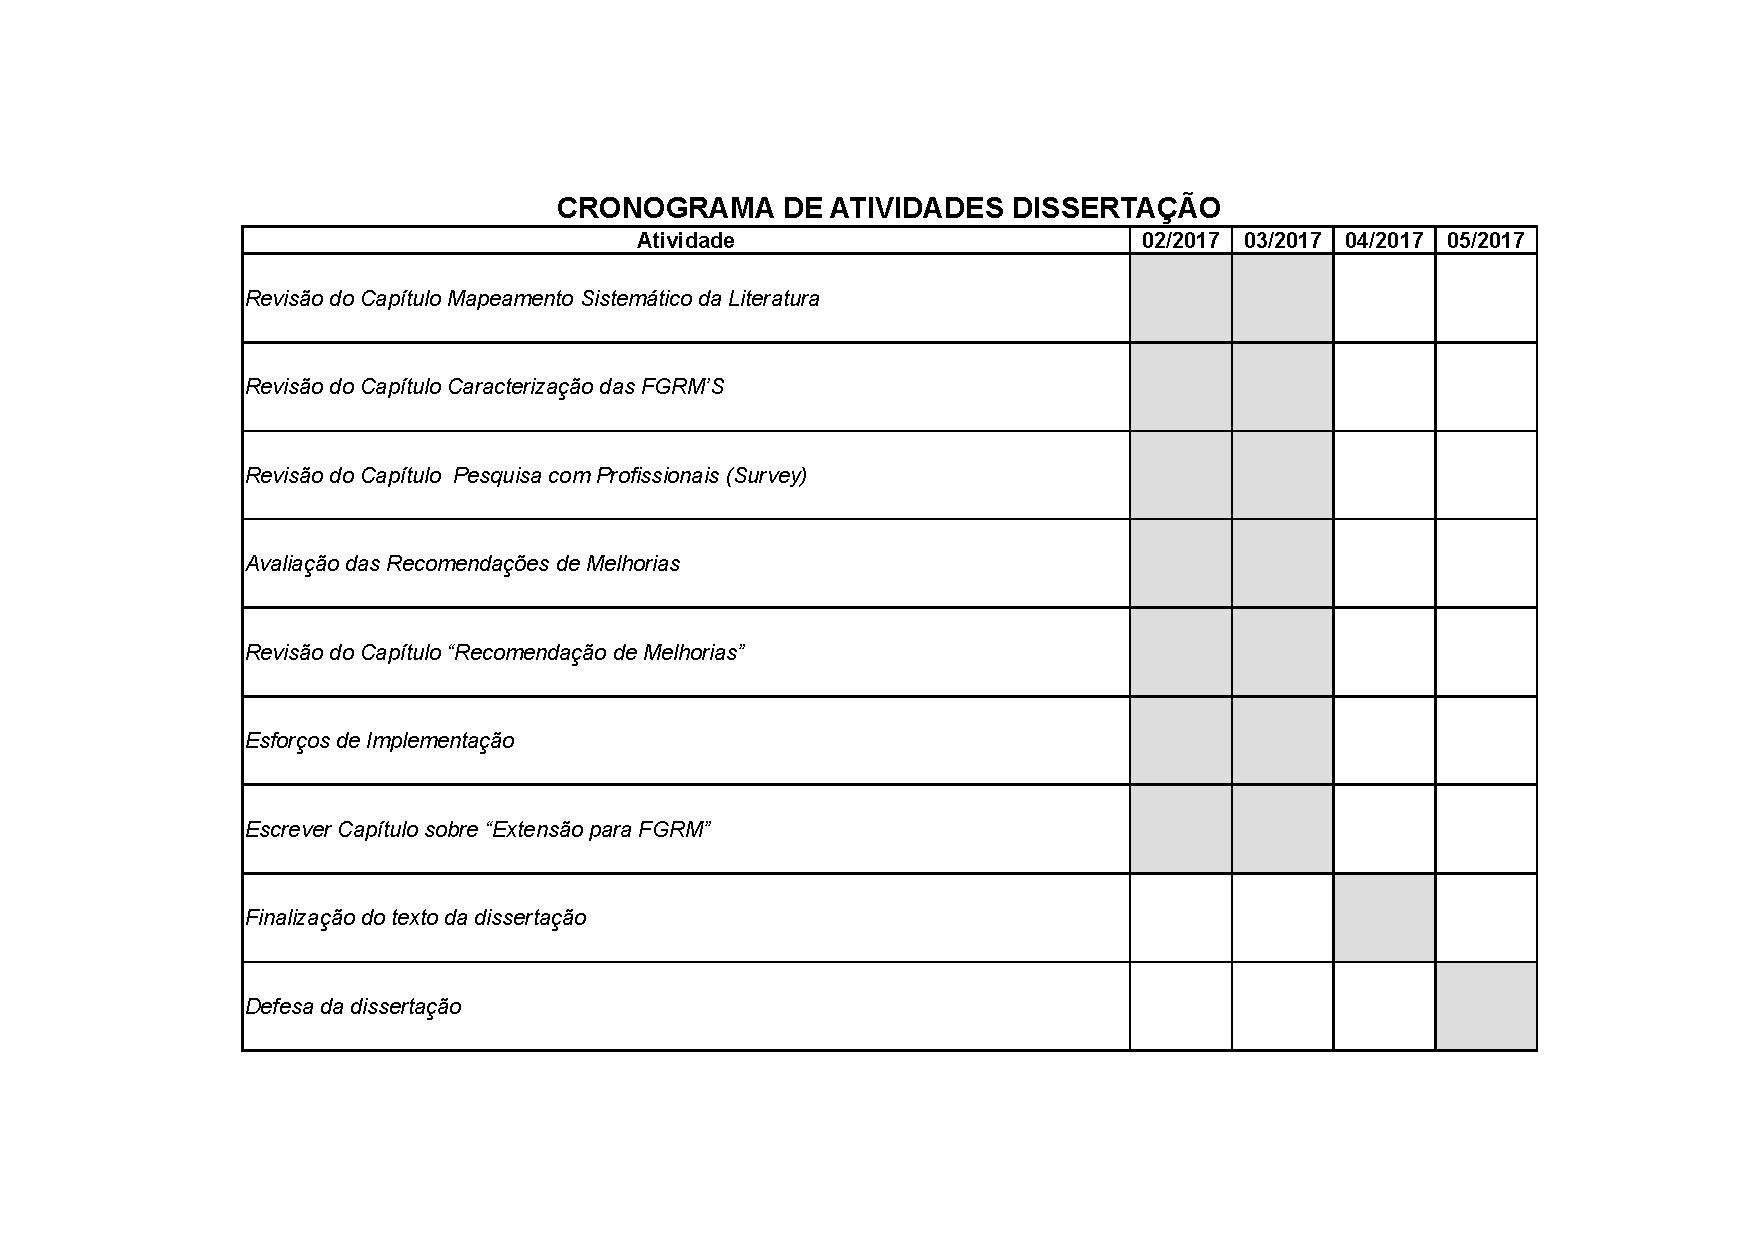
\includepdf{Cronograma-Atividades-Dissertacao.pdf}
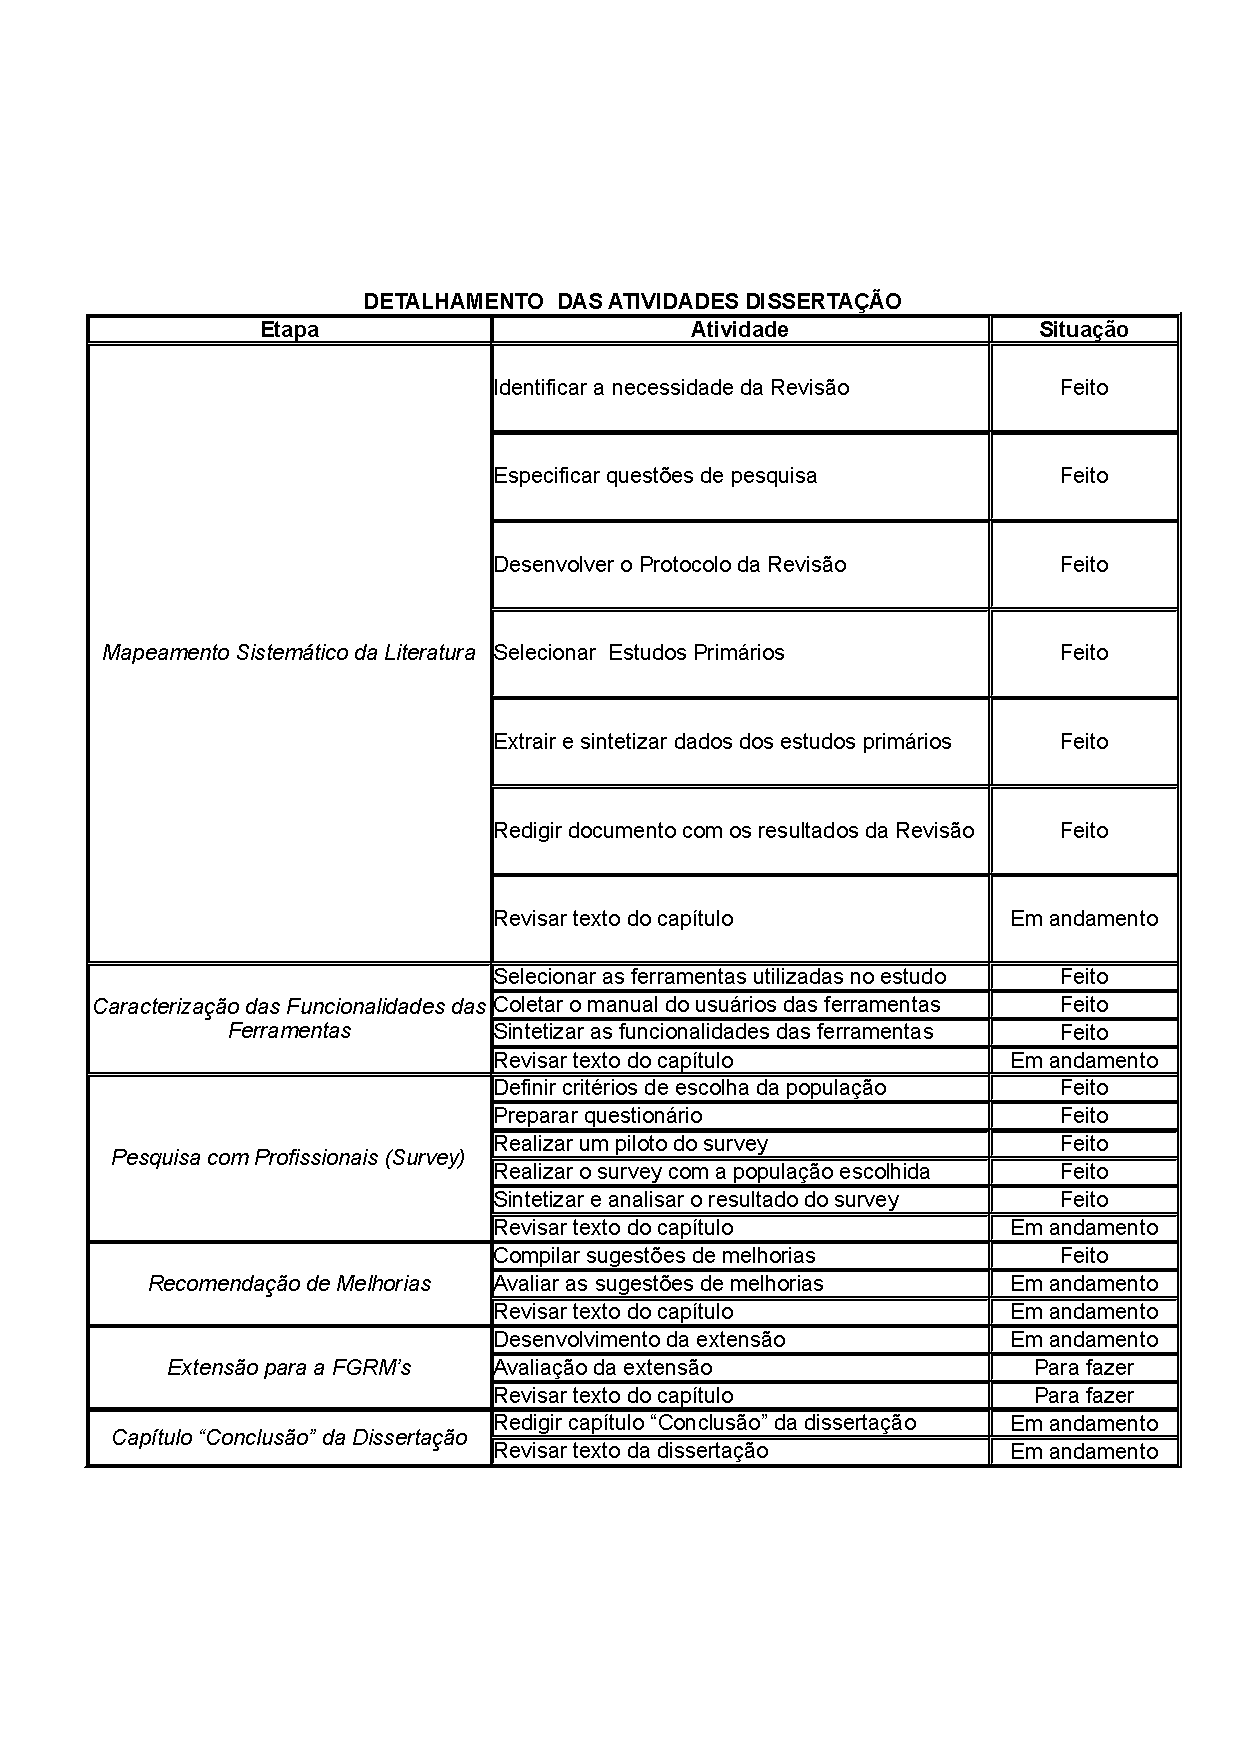
\includepdf{Detalhamento-Atividades-Dissertacao.pdf}

\bibliographystyle{acm}
\bibliography{relatorio}
\end{document}